Recall the statement, involving a simple matroid $\M$
with lattice of flats $\L=\L_\M$, a choice of a building
set $\G \subset \L \setminus \{\hat{0}\}$ that
contains $\hat{1}=E \in \G$, a subgroup $G \subseteq \Aut(\L)$,
for which $\G$ is setwise $G$-stable, and which satisfies the
{\it stabilizer condition} \eqref{eq:stabilizer-condition}:
\begin{quote}
 for any $\G$-nested set
   $N=\{F_i\}_{i=1,\ldots,\ell}$, if $g \in G$  has 
    $g(N)=N$, then $g(F_i)=F_i$ for $i=1,\ldots,\ell.$
\end{quote}



The statement also uses
the $\Z$-basis of FY-monomials for the Chow ring
$A(\L, \G)$ from Corollary~\ref{cor: mon_basis}:
$$
\fy:=\left\{x_{F_1}^{m_1}  \cdots x_{F_\ell}^{m_\ell} \colon
N:=\{F_1, \cdots,  F_\ell\} \text{ is } \G\text{-nested, and } 
0 \leq m_i < m_N(F_i) \text{ for }i=1,2,\ldots,\ell.\right\}
$$
where $m_N(F):=\rk(F)-\rk(\vee N_{<F})$ was defined in the Introduction (and repeated in \eqref{crucial-quantity}).


\vskip.1in
\noindent
{\bf Theorem~\ref{main-theorem}.}
{\it 
In the above context, there exist
\begin{itemize}
\item[(i)]
$\subgroup$-equivariant  bijections 
$
\pi: \FY^k  \overset{\sim}{\longrightarrow}  \FY^{r-k}
$ for $k \leq \frac{r}{2}$, and
\item[(ii)]
$\subgroup$-equivariant injections
$
\lambda: \FY^k  \hookrightarrow  \FY^{k+1}
$
for $k < \frac{r}{2}$.
\end{itemize}
}
\vskip.1in

%\begin{remark}
%One general instance where Theorem~\ref{main-theorem} applies is for the maximal building set $\G=\G_{\max}$.
%, and also for the minimal building set when $\G=\G_{\min}$ when $\L=\L_\M$ for a {\it connected matroid} $\M$, meaning that $E=\hat{1}$ is an indecomposable element in $\L.$
%\end{remark}


\begin{proof}[Proof of Theorem~\ref{main-theorem}]

The proof proceeds in these four steps:

\begin{itemize}
\item[{\sf Step 1.}]
    We first segregate the set of all of all $\FY$-monomials 
into the fibers of an {\it extended support} map
$$
\supp_+: \FY \rightarrow \N(\L,\G)
$$
defined as follows: if $m_i \geq 1$ for $1 \leq i \leq \ell$,
then
$$
\supp_+(x_{F_1}^{m_1} x_{F_2}^{m_2} \cdots x_{F_\ell}^{m_\ell})
:=\{F_1,\ldots,F_\ell\} \cup \{E\}.
$$ 
One of these fibers of $\supp_+$ is depicted in Example~\ref{extended-support-map-example} below.

\item[{\sf Step 2.}]
We check that for each 
$\G$-nested set $N^+=\{F_1,\ldots,F_\ell,E\}$ in the image of $\supp_+$,
the fiber $\supp_+^{-1}(N^+)$
is a collection of monomials which, when ordered by divisibility, forms a {\it Cartesian product of (saturated) chains}.  We also check, via Lemma~\ref{lem:crucial-numerical-fact}, that the degrees of the monomials in the fiber $\supp_+^{-1}(N^+)$ occupy a {\it symmetrically placed} interval $\{\ell,\ell+1,\ldots,(r-\ell)-1,r-\ell\}$
within the range of degrees $\{0,1,\ldots,r-1,r\}$ for the whole Chow ring $A(\L,\G)$.

\item[{\sf Step 3.}]
We check that the stabilizer condition \eqref{eq:stabilizer-condition} allows one to choose the identifications from {\sf Step 2} of
$\supp_+^{-1}(N^+)$ with Cartesian products of
chains {\it $G$-equivariantly} in a certain well-defined sense.

\item[{\sf Step 4.}]
Lastly, we show how the desired bijections $\pi$ and injections $\lambda$ on $\FY$-monomials can be pulled back from the corresponding self-dualities
and order-raising maps on the Cartesian products of chains.  The latter maps are derived from fixed {\it symmetric chain decompositions}, and
are checked to pull back to $G$-equivariant maps on the $\FY$-monomials, using the $G$-equivariance from {\sf Step 3}.

\end{itemize}

We now embark on the proof.
\vskip.1in
\noindent
{\sf Step 1.}\\
As in the outline, segregate the set of all $\FY$-monomials 
into the fibers of the {\it extended support} map
$$
\supp_+: \FY \rightarrow \N(\L,\G)
$$
defined as follows: if $m_i \geq 1$ for $1 \leq i \leq \ell$,
then
$$
\supp_+(x_{F_1}^{m_1} x_{F_2}^{m_2} \cdots x_{F_\ell}^{m_\ell})
:=\{F_1,\ldots,F_\ell\} \cup \{E\}.
$$ 
Note by Definition~\ref{def:nested-sets} of $\G$-nested sets
that, since $N=\{F_1,\ldots,F_\ell\}$ is $\G$-nested,
so is $N \cup \{E\}$. 

\vskip.1in
\noindent
{\sf Step 2.}\\
By the definition of $\fy$ in Corollary~\ref{cor: mon_basis}, a typical $\G$-nested set $N^+=\{F_1,\ldots,F_\ell,E\}$ in the image of $\supp_+$ 
has the following description for its fiber: 
$
\supp_+^{-1}(N^+) =\{
x_{F_1}^{m_1} x_{F_2}^{m_2} \cdots x_{F_\ell}^{m_\ell} x_E^{m_{\ell}+1}
\}
$
where the exponents on the monomials satisfy these inequalities:
\begin{equation}
    \label{fiber-inequalities}
\begin{aligned} 
&1 \leq m_{i} \leq m_{N^+}(F_i)-1 \text{ for }1\leq i \leq \ell,\\
&0 \leq m_{\ell+1} \leq m_{N^+}(E) - 1.
\end{aligned}
\end{equation}
As a consequence, the degrees of monomials
in the fiber $\supp_+^{-1}(N^+)$ lie in the range $[\ell,r-\ell]$: 
\begin{itemize}
    \item the minimum degree is achieved by $\deg(x_{F_1}^1 \cdots x_{F_\ell}^1 x_{E}^0)=\ell$, and
    \item the
maximum degree is achieved by
\begin{align*}
\deg\left(x_{F_1}^{m_{N^+}(F_1)-1} 
           \cdots x_{F_\ell}^{m_{N^+}(F_\ell)-1}
             x_{E}^{m_{N^+}(E)-1} \right)
&= \sum_{F \in N^+} (m_{N^+}(F)-1)\\
&= \rk(\vee N^+) - |N^+| \quad \text{ using Lemma~\ref{lem:crucial-numerical-fact},}\\
&= (r+1)-(\ell+1)=r-\ell. 
\end{align*}
\end{itemize}
Note also that the set of monomials in each such fiber $\supp_+^{-1}(N^+)$, when ordered via divisibility,
gives a poset isomorphic to a Cartesian product of chains
\begin{equation}
    \label{typical-product-of-chains}
\supp_+^{-1}(N^+) \cong C_{m_{N^+}(F_1)-1} \times 
C_{m_{N^+}(F_2)-1} \times \cdots \times
C_{m_{N^+}(F_\ell)-1} \times
C_{m_{N^+}(E)},
\end{equation}
where $C_m$ denotes a chain (totally ordered set) of size $m$.


\vskip.1in
\noindent
{\sf Step 3.}\\
In order to pin down a choice of the poset isomorphism in \eqref{typical-product-of-chains}, for each $\G$-nested set $N^+=\{F_1,\ldots,F_\ell,E\}$ in the image of $\supp_+$,
one must choose a linear order $(F_1,\ldots,F_\ell)$. It will be important
for the proof that these choices of linear order are {\it $G$-equivariant} in the 
following sense: whenever one has two $\G$-nested sets $N$ and $N'$ with chosen
linear orders $(F_1,F_2,\ldots,F_\ell)$ and $(F_1',F_2',\ldots,F_\ell')$, if
$g \in G$ has $g(N)=N'$, then one also has $g(F_i)=F_i'$ for $i=1,2,\ldots,\ell$. 
The fact that such a $G$-equivariant choice is possible follows from the stabilizer condition \eqref{eq:stabilizer-condition}:  one can choose the linear order $(F_1,\ldots,F_\ell)$ arbitrarily
on one $G$-orbit representative $N=\{F_1,\ldots,F_\ell\}$ from each $G$-orbit of $\G$-nested sets,
and then for any other element $g(N)$ within the orbit, decree its linear order to
be $(g(F_1),\ldots,g(F_\ell))$.  Condition \eqref{eq:stabilizer-condition} ensures that this is well-defined, independent of $g$: if $g,h \in G$ have $g(N)=h(N)$, then $g^{-1}h(N)=N$, so $g^{-1}h(F_i)=F_i$ and $g(F_i)=h(F_i)$ for
$i=1,\ldots,\ell$.


\vskip.1in
\noindent
{\sf Step 4.}\\
We now use the fact that
every ranked poset $P$ of rank $R$ which is a product of chains has a {\it symmetric chain decomposition (SCD)},
meaning a disjoint decomposition $P=\bigsqcup_{i=1}^t P_i$
    in which each $P_i$ is a chain passing through ranks $\{\rho_i,\rho_i+1,\ldots,R-\rho_i-1,R-\rho_i\}$ for some $\rho_i \in \{0,1,2,\ldots,\lfloor \frac{R}{2}\rfloor \}$;
    see, e.g., Anderson \cite[\S 3.1]{Anderson}.
Fix one such SCD for each product poset on the right side in \eqref{typical-product-of-chains}, which together with the choice of linear orders $(F_1,\ldots,F_
\ell)$, will induce an SCD on each fiber poset $\supp_+^{-1}\{F_1,\ldots,F_\ell,E\}$.  
An important point for the remainder of the proof
is that the structure of these symmetric chains depend only upon
the the linear orders $(F_1,\ldots,F_\ell)$ and numerical sequences 
$(m_{N^+}(F_1),  m_{N^+}(F_2),
\ldots,
m_{N^+}(F_\ell),
m_{N^+}(E))$, rather than depending upon finer information about the $\G$-nested set $N^+$.



\begin{example} \rm
\label{extended-support-map-example}
Let $\L=\L_\M$ be the lattice flats of a simple matroid $\M$ having $\rk(E)=10=r+1$ with $r=9$, and $\G=\G_{\max}$.  Consider
a $\G$-nested set $N^+=\{F_1,F_2,E\}$ where $F_1 < F_2$ are flats with $\rk(F_1)=3, \rk(F_2)=7$.  Linearly ordering $\{F_1,F_2\}$ as $(F_1,F_2)$, then the
divisibility poset on the fiber $\supp_+^{-1}\{F_1,F_2,E\}$ and one choice of SCD look as follows: 

%\robbie{Maybe we should stop using `nested' to refer to containment of flats, to avoid confusion with nested sets.} \a{agreed, changing it}


\begin{center}
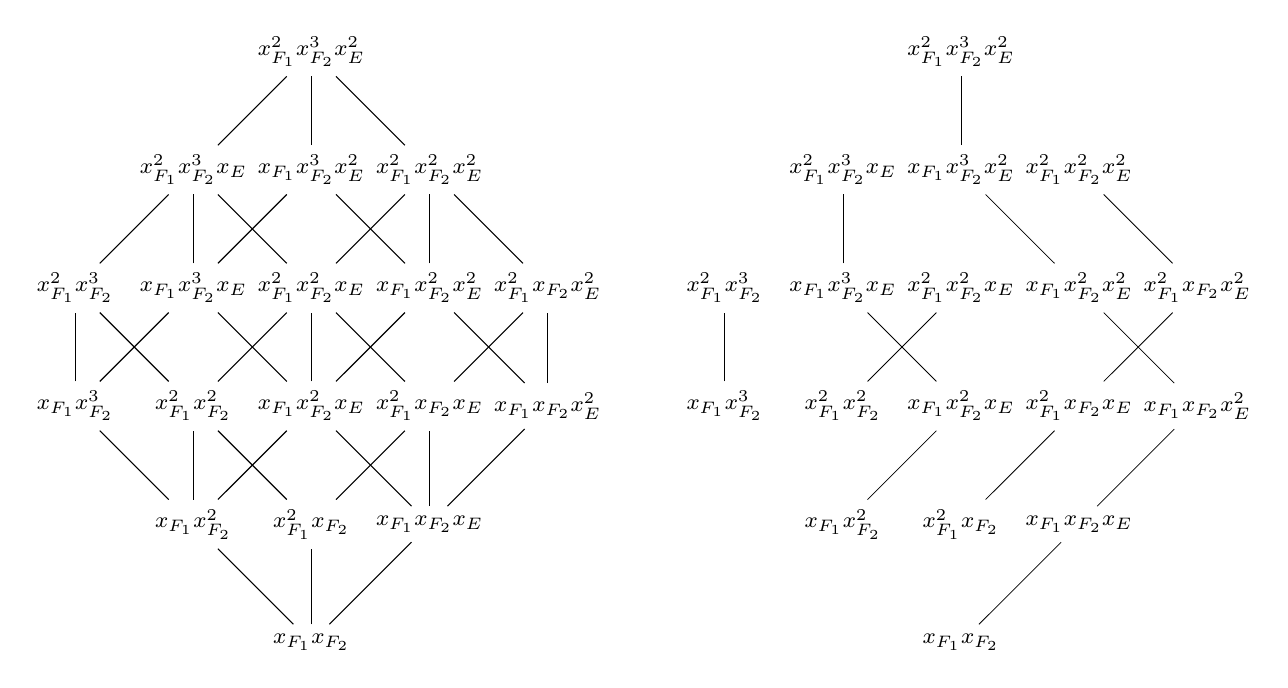
\begin{tikzpicture}
  [scale=.25,auto=left]
   \node (110) at (-6,0) {\footnotesize $x_{F_1} x_{F_2}$};
  \node (120) at (-12,6) {\footnotesize $x_{F_1} x_{F_2}^2$};
  \node (210) at (-6,6) {\footnotesize $x_{F_1}^2 x_{F_2}$};
  \node (111) at (0,6) {\footnotesize $x_{F_1} x_{F_2} x_E$};
  \node (130) at (-18,12) {\footnotesize $x_{F_1} x_{F_2}^3$};
  \node (220) at (-12,12) {\footnotesize $x_{F_1}^2 x_{F_2}^2$};
  \node (121) at (-6,12) {\footnotesize $x_{F_1} x_{F_2}^2 x_E$};
  \node (211) at (0,12) {\footnotesize $x_{F_1}^2 x_{F_2} x_E$};
  \node (112) at (6,12) {\footnotesize $x_{F_1} x_{F_2} x_E^2$};
  \node (230) at (-18,18) {\footnotesize $x_{F_1}^2 x_{F_2}^3$};
  \node (131) at (-12,18) {\footnotesize $x_{F_1} x_{F_2}^3 x_E$};
  \node (221) at (-6,18) {\footnotesize $x_{F_1}^2 x_{F_2}^2 x_E$};
  \node (122) at (0,18) {\footnotesize $x_{F_1} x_{F_2}^2 x_E^2$};
  \node (212) at (6,18) {\footnotesize $x_{F_1}^2 x_{F_2} x_E^2$};
  \node (231) at (-12,24) {\footnotesize $x_{F_1}^2 x_{F_2}^3 x_E$};
  \node (132) at (-6,24) {\footnotesize $x_{F_1} x_{F_2}^3 x_E^2$};
  \node (222) at (0,24) {\footnotesize $x_{F_1}^2 x_{F_2}^2 x_E^2$};
   \node (232) at (-6,30) {\footnotesize $x_{F_1}^2 x_{F_2}^3 x_E^2$};
  \foreach \from/\to in {110/120,110/210,110/111,  120/130,120/220,120/121,210/220,210/211,111/211,111/121,111/112,
130/230,130/131,220/230,220/221,121/221,121/131,211/221,211/212,112/122,112/212,121/122,
230/231,131/231,221/231,131/132,221/222,122/132,212/222,122/222,
    231/232,132/232,222/232}
    \draw (\from) -- (\to);
  [scale=.25,auto=left,every node]%/.style={circle,fill=black!20}]
   \node (110) at (27,0) {\footnotesize $x_{F_1} x_{F_2}$};
  \node (120) at (21,6) {\footnotesize $x_{F_1} x_{F_2}^2$};
  \node (210) at (27,6) {\footnotesize $x_{F_1}^2 x_{F_2}$};
  \node (111) at (33,6) {\footnotesize $x_{F_1} x_{F_2} x_E$};
  \node (130) at (15,12) {\footnotesize $x_{F_1} x_{F_2}^3$};
  \node (220) at (21,12) {\footnotesize $x_{F_1}^2 x_{F_2}^2$};
  \node (121) at (27,12) {\footnotesize $x_{F_1} x_{F_2}^2 x_E$};
  \node (211) at (33,12) {\footnotesize $x_{F_1}^2 x_{F_2} x_E$};
  \node (112) at (39,12) {\footnotesize $x_{F_1} x_{F_2} x_E^2$};
  \node (230) at (15,18) {\footnotesize $x_{F_1}^2 x_{F_2}^3$};
  \node (131) at (21,18) {\footnotesize $x_{F_1} x_{F_2}^3 x_E$};
  \node (221) at (27,18) {\footnotesize $x_{F_1}^2 x_{F_2}^2 x_E$};
  \node (122) at (33,18) {\footnotesize $x_{F_1} x_{F_2}^2 x_E^2$};
  \node (212) at (39,18) {\footnotesize $x_{F_1}^2 x_{F_2} x_E^2$};
  \node (231) at (21,24) {\footnotesize $x_{F_1}^2 x_{F_2}^3 x_E$};
  \node (132) at (27,24) {\footnotesize $x_{F_1} x_{F_2}^3 x_E^2$};
  \node (222) at (33,24) {\footnotesize $x_{F_1}^2 x_{F_2}^2 x_E^2$};
   \node (232) at (27,30) {\footnotesize $x_{F_1}^2 x_{F_2}^3 x_E^2$};
  \foreach \from/\to in {110/111,
  120/121,210/211,111/112,
130/230,220/221,121/131,211/212,112/122,
131/231,122/132,212/222,
132/232}
    \draw[line width=0.1mm] (\from) -- (\to);
\end{tikzpicture} 
\end{center}
\end{example}

We can now define the maps $\pi, \lambda$ asserted in the theorem.
Let $a$ be any FY-monomial $a$ with $k:=\deg(a)$.  Then $a$ lies in a unique fiber 
$\supp_+^{-1}(N^+)$ for some $\G$-nested set 
$N^+=\{F_1,\ldots,F_\ell,E\}$
of the map $\supp_+$, and on a unique chain $C_i$
in our fixed SCD of this fiber.  Writing 
\begin{equation}
\label{typical-SCD-chain}
C_i=\{ a_{\rho} \lessdot a_{\rho+1} \lessdot \cdots \lessdot a_{r-\rho-1} \lessdot a_{r-\rho} \},
\end{equation}
where $\deg(a_j)=j$ for $j=\rho,\rho+1,\ldots,r-\rho$,
so that $a=a_k$, then define the bijection $\pi$ and maps $\lambda$ via
\begin{align}
\label{pi-def}
\pi(a)&:=a_{r-k},\\
\label{lambda-def}
\lambda(a)&:=a_{k+1} \text{ if }k < \frac{r}{2}.
\end{align}
It remains to show that $\pi,\lambda$ are $\subgroup$-equivariant. Note that having fixed $N^+=\{F_1,\ldots,F_\ell,F_{\ell+1}:=E\}$,
both maps $f=\pi, \lambda$ will
map a monomial of the form $a=\prod_{i=1}^{\ell+1} x_{F_i}^{m_i}$
with $m_i \geq 1$ for $1 \leq i \leq \ell$ as follows:
$$
a=\prod_{i=1}^{\ell+1} x_{F_i}^{m_i}
\quad
\longmapsto 
\quad
f(a)=\prod_{i=1}^{\ell+1} x_{F_i}^{m'_i}
$$
where the exponents $(m'_1,\ldots,m'_\ell,m'_{\ell+1})$
are determined in \eqref{pi-def}, \eqref{lambda-def} uniquely by
our choice of linear ordering $(F_1,\ldots,F_\ell)$ and
by the data 
$$
\left( 
\,\,
(m_1,\ldots,m_{\ell},m_{\ell+1}) 
\,\,
,
\,\,
(m_{N^+}(F_1),  m_{N^+}(F_2),
\ldots,
m_{N^+}(F_\ell),
m_{N^+}(F_{\ell+1}))
\,\,
\right).
$$
Recall from the proof of Corollary~\ref{Chow-ring-carries-perm-reps-cor} that $g$ in $\subgroup$
have $m_{g(N)}(g(F))=m_{N}(F)$.  Also, our $G$-equivariant choice of linear orderings dictates that $g(N^+)=\{g(F_1),\ldots,g(F_\ell),E\}$ has linear order $(g(F_1),\ldots,g(F_\ell))$.  Thus either map $f=\pi, \lambda$ sends
$$
g(a)=\prod_{i=1}^{\ell+1} x_{g(F_i)}^{m_i}
\quad
\longmapsto 
\quad
f(g(a))= \prod_{i=1}^{\ell+1} x_{g(F_i)}^{m'_i}
=g(f(a)). \qedhere
$$
\end{proof}

\begin{remark}\rm \label{rmk:conclusion-failure}
Theorem~\ref{main-theorem} can fail without the
assumption of the stabilizer condition \eqref{eq:stabilizer-condition}. To see that this is true, consider the graphic matroid associated to a complete graph on $12$ vertices, with lattice of flats $\Pi_{12}$ and minimal building set $\G_{\min}$ (see Example~\ref{partition-lattice-example}). For this building set, the stabilizer condition \eqref{eq:stabilizer-condition} does not hold. For example, we have the following nested set 
    \begin{align*}
    N = \{F_1, F_2, F_3\}, \text{ where } F_1 &= 1,2,3,4|5|6|7|8|9|10|11|12, \\
    F_2 &= 5,6,7,8|1|2|3|4|9|10|11|12, \\ 
    \text{ and } F_3 &= 9,10,11,12|1|2|3|4|5|6|7|8.
    \end{align*}
The set $N$ is nested because the join $F_1 \vee F_2 \vee F_3 = 1,2,3,4|5,6,7,8|9,10,11,12$ has multiple non-singleton blocks, and is therefore not a member of $\G_{\min}$. The permutation $g = (1,5,9)(2,6,10)(3,7,11)(4,8,12)$ in $\symm_{12}$, expressed here in cycle notation, fixes $N$ setwise, but not pointwise:
it sends $F_1 \mapsto F_2 \mapsto F_3 \mapsto F_1$.

% Using $G=\symm_{12}$ one has the $\G_{\min}$-nested set 
% from Example~\ref{ex:maximal-and-minimal-versus-hypotheses},
% $N = \{F_1, F_2, F_3\}$ stabilized setwise but not pointwise, where
%     \begin{align*}
%     F_1 &= 1,2,3,4|5|6|7|8|9|10|11|12, \\
%     F_2 &= 5,6,7,8|1|2|3|4|9|10|11|12, \\ 
%     \text{ and } F_3 &= 9,10,11,12|1|2|3|4|5|6|7|8.
%     \end{align*}

Let us see how the conclusion of Theorem~\ref{main-theorem} also fails in this case. Here $N^+=\{F_1,F_2,F_3, E\}$ and each of the $F_i$ is of rank $3$ in $\Pi_{12}$, so $m_{N^+}(F_i)=3$. The join $F_1 \vee F_2 \vee F_3$ is of rank $9$, while the maximal element $E$ has rank $11$; thus we have $m_{N^+}(E)=2$. Following the proof of Theorem~\ref{main-theorem}, we have a poset isomorphism $\supp_+^{-1}(N^+) \cong C_2 \times C_2 \times C_2 \times C_2$:

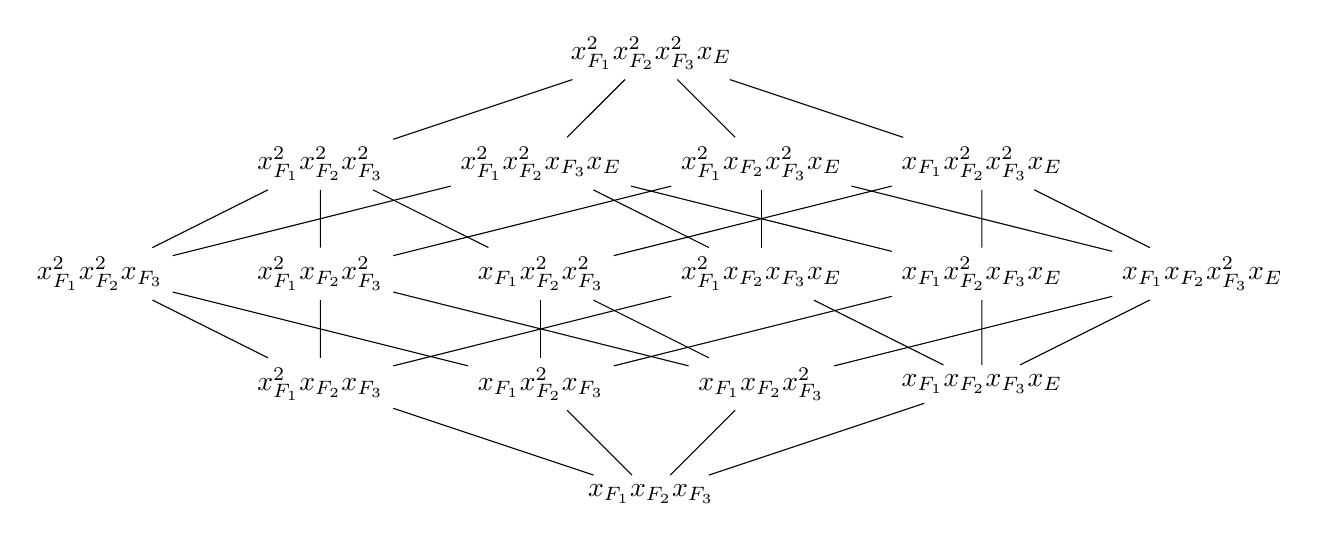
\begin{tikzpicture} [scale=.7,auto=left]
  \node (0) at (0,0) {$x_{F_1} x_{F_2} x_{F_3}$};
  
  \node (f2gh) at (-6,2) {$x_{F_1}^2 x_{F_2} x_{F_3}$};
  \node (fg2h) at (-2,2) {$x_{F_1} x_{F_2}^2x_{F_3}$};
  \node (fgh2) at (2,2) {$x_{F_1} x_{F_2}x_{F_3}^2$};
  \node (fghe) at (6,2) {$x_{F_1} x_{F_2} x_{F_3}x_E$};
  
  \node (f2g2h) at (-10,4) {$x_{F_1}^2 x_{F_2}^2 x_{F_3}$};
  \node (f2gh2) at (-6,4) {$x_{F_1}^2 x_{F_2} x_{F_3}^2$};
  \node (fg2h2) at (-2,4) {$x_{F_1} x_{F_2}^2 x_{F_3}^2$};
  
  \node (f2ghe) at (2,4) {$x_{F_1}^2 x_{F_2} x_{F_3} x_E$};
  \node (fg2he) at (6,4) {$x_{F_1} x_{F_2}^2 x_{F_3} x_E$};
  \node (fgh2e) at (10,4) {$x_{F_1} x_{F_2} x_{F_3}^2 x_E$};

  \node (f2g2h2) at (-6,6) {$x_{F_1}^2 x_{F_2}^2 x_{F_3}^2$};  
  \node (f2g2he) at (-2,6) {$x_{F_1}^2 x_{F_2}^2 x_{F_3} x_E$};
  \node (f2gh2e) at (2,6) {$x_{F_1}^2 x_{F_2} x_{F_3}^2 x_E$};
  \node (fg2h2e) at (6,6) {$x_{F_1} x_{F_2}^2 x_{F_3}^2 x_E$};
  
  \node (1) at (0,8) {$x_{F_1}^2 x_{F_2}^2 x_{F_3}^2 x_E$}; 

  \foreach \from/\to in {0/f2gh, 0/fg2h, 0/fgh2, 0/fghe, 
  					f2gh/f2g2h, f2gh/f2gh2, f2gh/f2ghe, 
					fg2h/fg2h2, fg2h/f2g2h, fg2h/fg2he,
					fgh2/f2gh2, fgh2/fg2h2, fgh2/fgh2e,
					fghe/f2ghe, fghe/fg2he, fghe/fgh2e,
					f2g2h/f2g2h2, f2g2h/f2g2he,
					f2gh2/f2g2h2, f2gh2/f2gh2e,
					fg2h2/f2g2h2, fg2h2/fg2h2e,
					f2ghe/f2g2he, f2ghe/f2gh2e,
					fg2he/f2g2he, fg2he/fg2h2e,
					fgh2e/f2gh2e, fgh2e/fg2h2e,
					f2g2h2/1, f2g2he/1, f2gh2e/1, fg2h2e/1}
 		\draw (\from) -- (\to);  
\end{tikzpicture}


If Theorem~\ref{main-theorem} held in this case, there would be an injective $G$-equivariant map $\lambda: \FY^4 \to \FY^5$. Injective $G$-equivariant maps preserve stabilizer subgroups; in other words, for any $m \in \FY$, one has $g \cdot m = m$ if and only if $g \cdot \lambda(m) = \lambda(m)$. We explain here why in this particular case, that requirement cannot be met.

The monomial $x_{F_1} x_{F_2} x_{F_3}x_E$ has a stabilizer subgroup isomorphic to $\symm_3[\symm_4]$, the wreath product of $\symm_3$ and $\symm_4$. Concretely, this stabilizer subgroup is generated by permutations stabilizing each of $\{1,2,3,4\}$, $\{5,6,7,8\}$, and $\{9,10,11,12\}$ setwise, and also permutations which swap these sets `wholesale.'  One can check that all monomials in $\FY(\Pi_{12})$ which have this stabilizer lie in the above fiber $\supp^{-1}(N^+)$
of the extended support map. Thus when attempting to construct $\lambda$, the image $\lambda(x_{F_1} x_{F_2} x_{F_3}x_E)$ must lie among the degree $5$ monomials in $\supp_+^{-1}(N^+)$. However, none of these degree $5$ monomials have the same stabilizer subgroup $\symm_3[\symm_4]$ as $x_{F_1} x_{F_2} x_{F_3}x_E$. For example, the permutation $g = (1,5,9)(2,6,10)(3,7,11)(4,8,12)$ mentioned above fixes
$x_{F_1} x_{F_2} x_{F_3}x_E$, but none of the degree $5$ monomials.
\end{remark}

\begin{remark} \rm
The $\subgroup$-equivariant bijections 
$
\pi: \FY^k  \overset{\sim}{\longrightarrow}  \FY^{r-k}
$
for $k \leq \frac{r}{2}$
in the above proof have an extra property:  a monomial $a$ always divides its image $\pi(a)$.  If one does not insist on this property, then
one has the following simpler $\subgroup$-equivariant bijection: 
given
$
a=x_{F_1}^{m_1} x_{F_2}^{m_2} \cdots x_{F_\ell}^{m_\ell} x_E^{m_{\ell+1}}
$
in $\FY^k$ 
where $k \leq \frac{r}{2}$
lying in
$
\supp_+^{-1}(N^+)\{F_1,\ldots,F_\ell,E\},
$
where $N^+=
\{F_1,\ldots,F_\ell,E\}
$
so that the $m_i$ satisfy the inequalities \eqref{fiber-inequalities}, then map the FY-monomial $a$ to this 
FY-monomial in the same fiber:
$$
a'=x_{F_1}^{m_{N^+}(F_1)-m_1} x_{F_2}^{m_{N^+}(F_2)-m_2}  \cdots
x_{F_\ell}^{m_{N^+}(F_\ell)-m_\ell} 
x_E^{m_{N^+}(E)-1-m_{\ell+1}}.
$$
%where $m'_i=\rk(F_i)-\rk(F_{i-1})-m_i$ for $i=1,2,\ldots,\ell$ and $m'_{\ell+1}=r-\rk(F_\ell)-m_{\ell+1}$ with usual convention $F_0:=\varnothing$.  
The authors thank Connor Simpson for pointing out that the latter bijection is (up to a plus/minus sign) the specialization of a bijection appearing in the work of Pagaria and Pezzoli \cite[Defn.~4.3]{PagariaPezzoli}, where they produce an explicit Poincar\'e duality isomorphism for Chow rings of all {\it polymatroids}.
\end{remark}







In the remainder of this section, we explain
a combinatorial proof of Theorem \ref{main-theorem} that works only for the maximal building set $\G_{\max}$; it can be seen as a way of making concrete choices of the SCDs in the previous proof. Recall that the \textit{maximal} building set is $\G_\text{max} = \L \setminus \{\emptyset\}$. The nested sets in $\G_\text{max}$ are simply chains in $\L \setminus \{\hat{0}\}$ (see Section~\ref{building-set-basics}), and the Feichtner-Yuzvinsky monomials with respect to $\G_\text{max}$ have the form
    \[\fy := \left\{ x_{F_1}^{m_1} \cdot x_{F_2}^{m_2}\cdots x_{F_\ell}^{m_\ell}: \emptyset = F_0 \subsetneq F_1 \subsetneq \ldots \subsetneq F_\ell \text{ is a chain and } m_i < \rk(F_i) - \rk(F_{i-1}) \text{ for all } i \right\}.\]
This proof borrows an idea from the famous {\it parenthesis-pairing}
SCD of Boolean lattices due to Greene and Kleitman \cite{GK}.  We begin with a two-step encoding of FY-monomials within a fiber of the map $\supp_+$. 

\begin{defn} \rm
Consider all FY-monomials $a=x_{F_1}^{m_1} \cdots x_{F_\ell}^{m_\ell} x_E^{m_{\ell+1}}$ having a fixed extended support set
$\supp_+(a)=\{F_1 \subsetneq \cdots \subsetneq F_\ell \subsetneq F_{\ell+1}=E\}$, so $m_1,\ldots,m_\ell \geq 1$ and $m_{\ell+1} \geq 0$.  In the first step, encode such monomials
$a$ via
a sequence $\DD(a)$ of length $r$
in three symbols $\times, \bullet$, and a blank space, defined as follows:
\begin{itemize}
    \item $\DD(a)$ has $\bullet$ in the positions $\{\rk(F_1),\ldots,\rk(F_\ell)\}$.
\item  $\DD(a)$ has $\times$ in the first consecutive $m_i$ positions to the left of $\rk(F_i)$ for each $i=1,2,\ldots,\ell,\ell+1$.
\item $\DD(a)$ has a blank space in the remaining positions.
\end{itemize}

\begin{example} \label{dd-example}
\rm Continuing with the matroid $\M$ and its flats $F_1 < F_2$ as discussed in Example~\ref{extended-support-map-example}.  Here the monomials lie in the fiber
$\supp_+^{-1}\{F_1,F_2,E\}$ where 
$\{\rk(F_1),\rk(F_2),\rk(E)\}=\{3,7,10\}$, so $r=9$, and the positions $\{\rk(F_1),\rk(F_2)\}=\{3,7\}$ are shown in {\color{teal} teal}. The monomial $x_{F_1} x_{F_2}^2$ gets encoded as
\[\begin{array}{ccccccccc}
     1 & 2 & {\color{teal} 3} & 4 & 5 & 6 & {\color{teal} 7} & 8 & 9  \\ \\
      & \times & {\color{teal} \bullet} &  & \times & \times & {\color{teal} \bullet} &  & 
     %) & ( & ) & ) & ( & ( & ) & ) & )
\end{array}\]

    
\end{example}


\end{defn}

\noindent
Note that one can recover $a$ from 
$
\supp_+(a)=\{F_1,\ldots,F_\ell, E\}
$
and $\DD(a)$, since $m_i$ can be read off as the number of $\times$ in $\DD(a)$ between positions $\rk(F_{i-1})$ and $\rk(F_i)$, with usual conventions
$F_0=\varnothing, F_{\ell+1}:=E$.

\begin{defn} \rm
The second step encodes $\DD(a)$ as a length $r$ parenthesis sequence in $\{(,)\}^r$,  having \begin{itemize}
    \item a right parenthesis ``$)$" in the positions of each $\bullet$ and each blank space, and 
    \item a left parenthesis ``(" in the positions of the $\times$.
\end{itemize}

\end{defn}

\begin{example} \label{dd-to-()-example}
  \rm  Continuing Example~\ref{dd-example}, the diagram $\DD(x_{F_1} x_{F_2}^2)$ is encoded as this sequence of parentheses:
    \[\begin{array}{ccccccccc}
     1 & 2 & {\color{teal} 3} & 4 & 5 & 6 & {\color{teal} 7} & 8 & 9  \\ \\
      & \times & {\color{teal} \bullet} &  & \times & \times & {\color{teal} \bullet} &  & \\
     ) & ( & ) & ) & ( & ( & ) & ) & )
\end{array}\]
\end{example}

\noindent
Note that one can recover $\DD(a)$ from this
 $\{(,)\}^r$ sequence as follows: 
 \begin{itemize}
  \item[-]  $\DD(a)$ has $\times$ occurring in the positions of the left parentheses, and 
     \item[-] $\DD(a)$ has the $\bullet$ occurring
 exactly in the positions of the right parenthesis in a consecutive pair $()$, while blank spaces occur in the position of all other right parentheses.
 \end{itemize}

\begin{proof}[Second proof of Theorem~\ref{main-theorem} for $\G=\G_{\max}$.]

Given an FY-monomial $a$ in $\FY^k$ with $k \leq \frac{r}{2}$, we will use its parenthesis sequence in $\{(,)\}^r$ to place $a$ within a chain of monomials as in \eqref{typical-SCD-chain}, of
the form
$$
C_i=\{ a_{\rho} \lessdot a_{\rho+1} \lessdot \cdots \lessdot a_{r-\rho-1} \lessdot a_{r-\rho} \},
$$
where $\deg(a_j)=j$ for $j=\rho,\rho+1,\ldots,r-\rho$,
so that $a=a_k$.  To this end, define the set of {\it paired parentheses} in $a$ (shown underlined in Example~\ref{example-re-revisited})
by including all consecutive pairs $()$, and after removing these
consecutive pairs, including the new $()$ pairs which have become consecutive, repeating this recursively.  After removing some number $\rho$ of pairs $()$ via this pairing process, the process ends when one reaches a sequence of $r -2 \rho$ remaining unpaired parentheses of this form:
\begin{equation}
\label{unpaired-parentheses}
\underbrace{)) \cdots ))}_{k-\rho}
\underbrace{{\color{orange}(( \cdots ((}}_{r-\rho-k}.
\end{equation}
The monomials in the chain $C_i$ are defined to
be those whose set of paired parentheses agree
exactly with those of $a$, both in their postitions, and left-right pairing structure-- see the underlined parentheses in Example~\ref{example-re-revisited}.  

As in the first proof of Theorem~\ref{main-theorem}, one then defines the bijections $\pi$ and maps $\lambda$ via
$$
\begin{aligned}
\pi(a)&:=a_{r-k},\\
\lambda(a)&:=a_{k+1}  \text{ if }k < \frac{r}{2}.
\end{aligned}
$$
In other words, both maps $\lambda$ and $\pi$
when applied to $a$ will keep all of the paired parentheses fixed, but 
\begin{itemize}
    \item $\lambda$ changes the leftmost unpaired left parenthesis ``)" into an unpaired right parenthesis ``{\color{orange}(}", and
    \item $\pi$ swaps the numbers $k-\rho$ and $r-\rho-k$ of unpaired right and left parentheses in \eqref{unpaired-parentheses}.
\end{itemize}

The equivariance of these two maps $\pi, \lambda$ is argued exactly as in the first proof of the theorem.
\end{proof}


\begin{example}\rm
\label{example-re-revisited}
Here is an example of a symmetric chain from Example~\ref{extended-support-map-example},
explained via this two-step encoding with $\DD(a)$ and
$\{(,)\}^r$-sequences, as we have seen preceding Examples~\ref{dd-example} and ~\ref{dd-to-()-example}. 
Paired parentheses are underlined, and are fixed throughout the chain. Moving up the chain, unpaired right parentheses change one-by-one to left parentheses (depicted {\color{orange} orange} here), in order from right to left:


\small
$$
\begin{array}{ccccccccccl}
 & 1 & 2 & {\color{teal}3} & 4 & 5 & 6 & {\color{teal}7} & 8 & 9 \\
    &  &  &  &  &  &  &  &  &  \\
x_{F_1}^2 x_{F_2}^3 x_E & \times & \times & {\color{teal}\bullet} & \times & \times & \times &{\color{teal}\bullet}  &  & \times\\
& {\color{orange}(} & \underline{(} & \underline{)} & {\color{orange}(} & \underline{(} & \underline{(} & \underline{)} & \underline{)} & {\color{orange}(}\\ 
    &  &  &  &  &  &  &  &  &  \\
 \uparrow &  &  &  &  &  &  &  &  &  \\
    &  &  &  &  &  &  &  &  &  \\
x_{F_1} x_{F_2}^3 x_E &  & \times & {\color{teal}\bullet} & \times & \times & \times &{\color{teal}\bullet}  &  & \times\\
& ) & \underline{(} & \underline{)} & {\color{orange}(} & \underline{(} & \underline{(} & \underline{)} & \underline{)} & {\color{orange}(}\\ 
    &  &  &  &  &  &  &  &  &  \\
 \uparrow &  &  &  &  &  &  &  &  &  \\
    &  &  &  &  &  &  &  &  &  \\
x_{F_1} x_{F_2}^2 x_E &  & \times & {\color{teal}\bullet} &  & \times & \times &{\color{teal}\bullet}  &  & \times\\
& ) & \underline{(} & \underline{)} & ) & \underline{(} & \underline{(} & \underline{)} & \underline{)} & {\color{orange}(}\\ 
   &  &  &  &  &  &  &  &  &  \\
 \uparrow &  &  &  &  &  &  &  &  &  \\
    &  &  &  &  &  &  &  &  &  \\
x_{F_1} x_{F_2}^2 
 &  & \times & {\color{teal}\bullet} &   & \times & \times &{\color{teal}\bullet}  &  &  \\
 & ) & \underline{(} & \underline{)} & ) & \underline{(} & \underline{(} & \underline{)} & \underline{)} & )\\ 
\end{array}
$$
\normalsize


Here $r=9$ and the number of parenthesis pairs is $\rho=3$, so that this chain $C_i$ is symmetrically placed within the degrees of $A(\L_\M, \G_{\max})$, containing monomials of degrees $[\rho,r-\rho]=[3,6]=\{3,4,5,6\}$ 
out of the list of possible degrees $[0,r]=[0,9]=\{0,1,2,\mathbf{3,4,5,6},7,8,9\}$. 
\end{example}
